\begin{frame}{Metodologia}{Análise e definição das características do projeto}

  \begin{figure}[H]
    \centering
    \caption{Esquema de demonstração de uma cisterna no subsolo}
    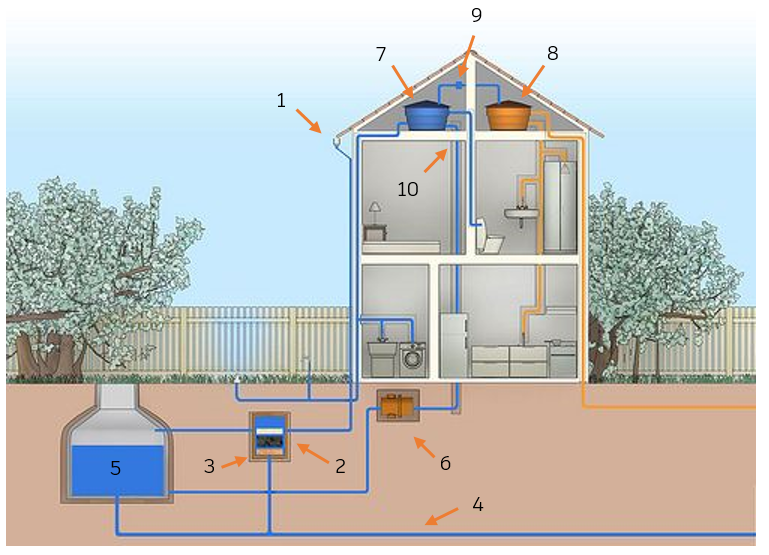
\includegraphics[width=0.6\textwidth]{figuras/esquema_cisterna.png}
    \caption*{Fonte: Adaptado (ECOMONTES, 2016)}
    \label{fig:esquema_cisterna}
  \end{figure}

\end{frame}

\begin{frame}{Metodologia}{Análise e definição das características do projeto}
 
  \begin{table}[]
    \hspace*{-3cm}
    \begin{centering}
    \resizebox{0.55\textwidth}{!}{\begin{minipage}{\textwidth}
    \begin{tabular}{c|c|c}
      \hline
      \textbf{Identificador} & \textbf{Elemento} & \textbf{Descrição} \\ \hline
      1 & Calha coletora & \begin{tabular}[c]{@{}c@{}}Elemento convencional para coleta e \\ descarte de água da chuva\end{tabular} \\ \hline
      2 & Filtro A (cascalho fino) & \begin{tabular}[c]{@{}c@{}}Elemento para realização de \\ filtragem de pequenas impurezas\end{tabular} \\ \hline
      3 & Filtro B (cascalho grosso) & \begin{tabular}[c]{@{}c@{}}Elemento para realização de \\ filtragem de impurezas\end{tabular} \\ \hline
      4 & Tubulação de descarte & \begin{tabular}[c]{@{}c@{}}Tubulação utilizada como rota de escoamento \\ quando o reservatório não está em uso ou \\ está cheio\end{tabular} \\ \hline
      5 & Reservatório de coleta & Cisterna propriamente dita \\ \hline
      6 & Motobomba ou bomda d'água & \begin{tabular}[c]{@{}c@{}}Elemento utilizado para realização do \\ ganho de elevação da água\end{tabular} \\ \hline
      7 & Caixa d'água auxiliar & \begin{tabular}[c]{@{}c@{}}Caixa d'água convencional com alimentação \\ oriunda da bomba d'água\end{tabular} \\ \hline
      8 & Caixa d'água convencional & \begin{tabular}[c]{@{}c@{}}Caixa d'água padrão com alimentação \\ da estação de água da cidade\end{tabular} \\ \hline
      9 & Elo de ligação & \begin{tabular}[c]{@{}c@{}}Ligação utilizada para abastecer a caixa d'água \\ auxiliar quando a cisterna está seca \\ ou em manutenção\end{tabular} \\ \hline
      10 & Distribuidor & \begin{tabular}[c]{@{}c@{}}Elementos de distribuição de água \\ para pontos estratégicos\end{tabular} \\ \hline
    \end{tabular}
    \caption{Identificação dos elementos da Figura \autoref{fig:esquema_cisterna}.}
  \end{minipage}}
  \end{centering}
  \end{table}

\end{frame}

\begin{frame}{}

  \begin{figure}[H]
    \vspace*{-0.3cm}
    \centering
    \caption{Esquema básico do projeto.}
    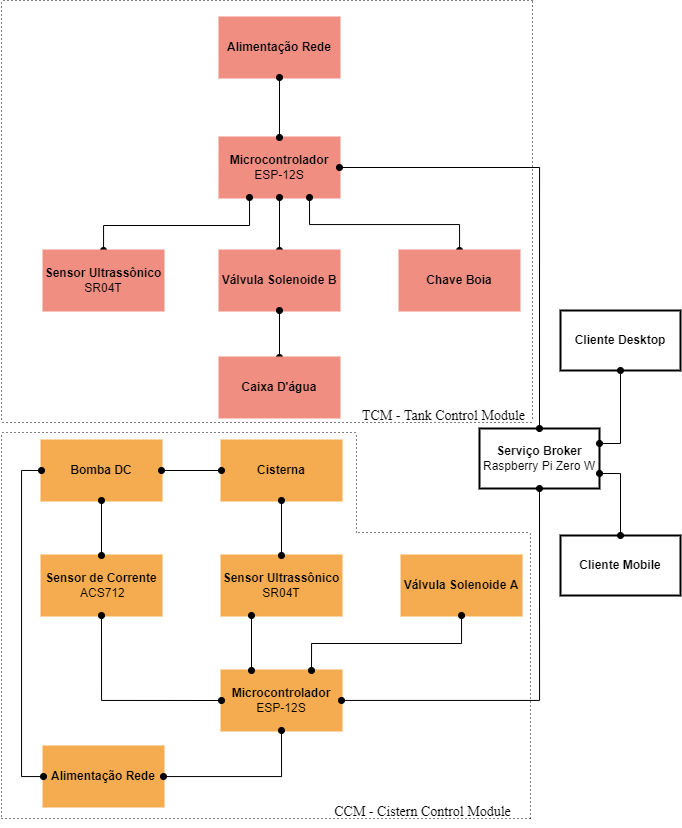
\includegraphics[width=0.5\textwidth]{figuras/esquema_basico_proj_2.png}
    \caption*{\small{Fonte: Própria}}
    \label{fig:esquema_proj}
    
  \end{figure}
  
\end{frame}